%-----------------------------------------------------------------------------------------------------------------------------------------------%
%   The MIT License (MIT)
%
%	Copyright (c) 2015 Jan Küster
%
%	Permission is hereby granted, free of charge, to any person obtaining a copy
%	of this software and associated documentation files (the "Software"), to deal
%	in the Software without restriction, including without limitation the rights
%	to use, copy, modify, merge, publish, distribute, sublicense, and/or sell
%	copies of the Software, and to permit persons to whom the Software is
%	furnished to do so, subject to the following conditions:
%	
%	THE SOFTWARE IS PROVIDED "AS IS", WITHOUT WARRANTY OF ANY KIND, EXPRESS OR
%	IMPLIED, INCLUDING BUT NOT LIMITED TO THE WARRANTIES OF MERCHANTABILITY,
%	FITNESS FOR A PARTICULAR PURPOSE AND NONINFRINGEMENT. IN NO EVENT SHALL THE
%	AUTHORS OR COPYRIGHT HOLDERS BE LIABLE FOR ANY CLAIM, DAMAGES OR OTHER
%	LIABILITY, WHETHER IN AN ACTION OF CONTRACT, TORT OR OTHERWISE, ARISING FROM,
%	OUT OF OR IN CONNECTION WITH THE SOFTWARE OR THE USE OR OTHER DEALINGS IN
%	THE SOFTWARE.
%	
%
%-----------------------------------------------------------------------------------------------------------------------------------------------%


%============================================================================%
%
%	DOCUMENT DEFINITION
%
%============================================================================%

%we use article class because we want to fully customize the page and dont use a cv template
\documentclass[10pt,A4]{article}	


%----------------------------------------------------------------------------------------
%	ENCODING
%----------------------------------------------------------------------------------------

%we use utf8 since we want to build from any machine
\usepackage[utf8]{inputenc}		

%----------------------------------------------------------------------------------------
%	LOGIC
%----------------------------------------------------------------------------------------

% provides \isempty test
\usepackage{xifthen}

%----------------------------------------------------------------------------------------
%	FONT
%----------------------------------------------------------------------------------------

% some tex-live fonts - choose your own

%\usepackage[defaultsans]{droidsans}
%\usepackage[default]{comfortaa}
%\usepackage{cmbright}
\usepackage[default]{raleway}
%\usepackage{fetamont}
%\usepackage[default]{gillius}
%\usepackage[light,math]{iwona}
%\usepackage[thin]{roboto} 

% set font default
\renewcommand*\familydefault{\sfdefault} 	
\usepackage[T1]{fontenc}

% more font size definitions
\usepackage{moresize}		

% line spacing
\usepackage{setspace}
\setstretch{1.2}

%----------------------------------------------------------------------------------------
%	PAGE LAYOUT  DEFINITIONS
%----------------------------------------------------------------------------------------

%debug page outer frames
%\usepackage{showframe}			


%define page styles using geometry
\usepackage[a4paper]{geometry}		

% for example, change the margins to 2 inches all round
\geometry{top=1.75cm, bottom=-.6cm, left=1.5cm, right=1.5cm} 	

%use customized header
\usepackage{fancyhdr}				
\pagestyle{fancy}

%less space between header and content
\setlength{\headheight}{-5pt}		


%customize entries left, center and right
\lhead{}
\chead{ \small{Pedro Moreira$\cdot$ Senior Software Engineer $\cdot$  Gent, Belgium  $\cdot$  \textcolor{sectcol}{\textbf{pedrogrmoreira@gmail.com}}  $\cdot$ +32 476 86 52 11}}
\rhead{}


%indentation is zero
\setlength{\parindent}{0mm}

%----------------------------------------------------------------------------------------
%	TABLE /ARRAY DEFINITIONS
%---------------------------------------------------------------------------------------- 

%for layouting tables
\usepackage{multicol}			
\usepackage{multirow}

%extended aligning of tabular cells
\usepackage{array}

\newcolumntype{x}[1]{%
>{\raggedleft\hspace{0pt}}p{#1}}%


%----------------------------------------------------------------------------------------
%	GRAPHICS DEFINITIONS
%---------------------------------------------------------------------------------------- 

%for header image
\usepackage{graphicx}

%for floating figures
\usepackage{wrapfig}
\usepackage{float}
%\floatstyle{boxed} 
%\restylefloat{figure}

%for drawing graphics		
\usepackage{tikz}				
\usetikzlibrary{shapes, backgrounds,mindmap, trees}


%----------------------------------------------------------------------------------------
%	Color DEFINITIONS
%---------------------------------------------------------------------------------------- 

\usepackage{color}

%accent color
\definecolor{sectcol}{RGB}{255,150,0}

%dark background color
\definecolor{bgcol}{RGB}{110,110,110}

%light background / accent color
\definecolor{softcol}{RGB}{225,225,225}


%============================================================================%
%
%
%	DEFINITIONS
%
%
%============================================================================%

%----------------------------------------------------------------------------------------
% 	HEADER
%----------------------------------------------------------------------------------------

% remove top header line
\renewcommand{\headrulewidth}{0pt} 

%remove botttom header line
\renewcommand{\footrulewidth}{0pt}	  	

%remove pagenum
\renewcommand{\thepage}{}	

%remove section num		
\renewcommand{\thesection}{}			

%----------------------------------------------------------------------------------------
% 	ARROW GRAPHICS in Tikz
%----------------------------------------------------------------------------------------

% a six pointed arrow poiting to the left
\newcommand{\tzlarrow}{(0,0) -- (0.2,0) -- (0.3,0.2) -- (0.2,0.4) -- (0,0.4) -- (0.1,0.2) -- cycle;}	

% include the left arrow into a tikz picture
% param1: fill color
%
\newcommand{\larrow}[1]
{\begin{tikzpicture}[scale=0.58]
	 \filldraw[fill=#1!100,draw=#1!100!black]  \tzlarrow
 \end{tikzpicture}
}

% a six pointed arrow poiting to the right
\newcommand{\tzrarrow}{ (0,0.2) -- (0.1,0) -- (0.3,0) -- (0.2,0.2) -- (0.3,0.4) -- (0.1,0.4) -- cycle;}

% include the right arrow into a tikz picture
% param1: fill color
%
\newcommand{\rarrow}
{
\begin{tikzpicture}[scale=0.7]
	\filldraw[fill=sectcol!100,draw=sectcol!100!black] \tzrarrow
 \end{tikzpicture}
}



%----------------------------------------------------------------------------------------
%	custom sections
%----------------------------------------------------------------------------------------

% create a coloured box with arrow and title as cv section headline
% param 1: section title
%
\newcommand{\cvsection}[1]
{
\colorbox{sectcol}{\mystrut \makebox[1\linewidth][l]{
\larrow{bgcol} \hspace{-8pt} \larrow{bgcol} \hspace{-8pt} \larrow{bgcol} \textcolor{white}{\textbf{#1}}\hspace{4pt}
}}\\
}

%create a coloured arrow with title as cv meta section section
% param 1: meta section title
%
\newcommand{\metasection}[2]
{
\begin{tabular*}{1\textwidth}{p{2.6cm} p{11cm}}
\larrow{bgcol}	\normalsize{\textcolor{sectcol}{#1}}&#2\\[6pt]
\end{tabular*}
}

%----------------------------------------------------------------------------------------
%	 CV EVENT
%----------------------------------------------------------------------------------------

% creates a stretched box as cv entry headline followed by paragraphs about 
% the work you did
% param 1:	event time i.e. 2014 or 2011-2014 etc.
% param 2:	event name (what did you do?)
% param 3:	institution (where did you work / study)
% param 4:	what were your positions
%
\newcommand{\cvevent}[4]
{
	\begin{tabular*}{1\textwidth}{p{2.3cm}  p{10.9cm} x{3.8cm}}
 \textcolor{bgcol}{#1}& \textbf{#2} & \vspace{2.5pt}\textcolor{sectcol}{#3}

	\end{tabular*}
\vspace{-12pt}
\textcolor{softcol}{\hrule}
\vspace{6pt}
	\ifthenelse{\equal{#4}{}}{}{
		\begin{tabular*}{1\textwidth}{p{2.3cm} p{14.4cm}}
			& \foreach \x in {#4} {
				\larrow{bgcol}~\x\par\vspace{3pt}
			}
		\end{tabular*}
	}
}

% creates a stretched box as 
\newcommand{\cveventmeta}[2]
{
	\mbox{\mystrut \hspace{87pt}\textit{#1}}\\
	#2
}

%----------------------------------------------------------------------------------------
% CUSTOM STRUT FOR EMPTY BOXES
%----------------------------------------- -----------------------------------------------
\newcommand{\mystrut}{\rule[-.3\baselineskip]{0pt}{\baselineskip}}

%----------------------------------------------------------------------------------------
% CUSTOM LOREM IPSUM
%----------------------------------------------------------------------------------------
\newcommand{\lorem}
{Lorem ipsum dolor sit amet, consectetur adipiscing elit. Donec a diam lectus.}



%============================================================================%
%
%
%
%	DOCUMENT CONTENT
%
%
%
%============================================================================%
\begin{document}


%use our custom fancy header definitions
\pagestyle{fancy}	


%---------------------------------------------------------------------------------------
%	TITLE HEADLINE
%----------------------------------------------------------------------------------------
\vspace{-20.55pt}

% use this for single words, e.g. CV or RESUME etc.
\hspace{-0.25\linewidth}\colorbox{bgcol}{\makebox[1.5\linewidth][c]{\HUGE{\textcolor{white}{\textsc{Pedro Moreira}} } \textcolor{sectcol}{\rule[-1mm]{1mm}{0.9cm}} \HUGE{\textcolor{white}{\textsc{Resume}} } }}


%----------------------------------------------------------------------------------------
%	HEADER IMAGE
%----------------------------------------------------------------------------------------

\begin{figure}[H]
\begin{flushright}
	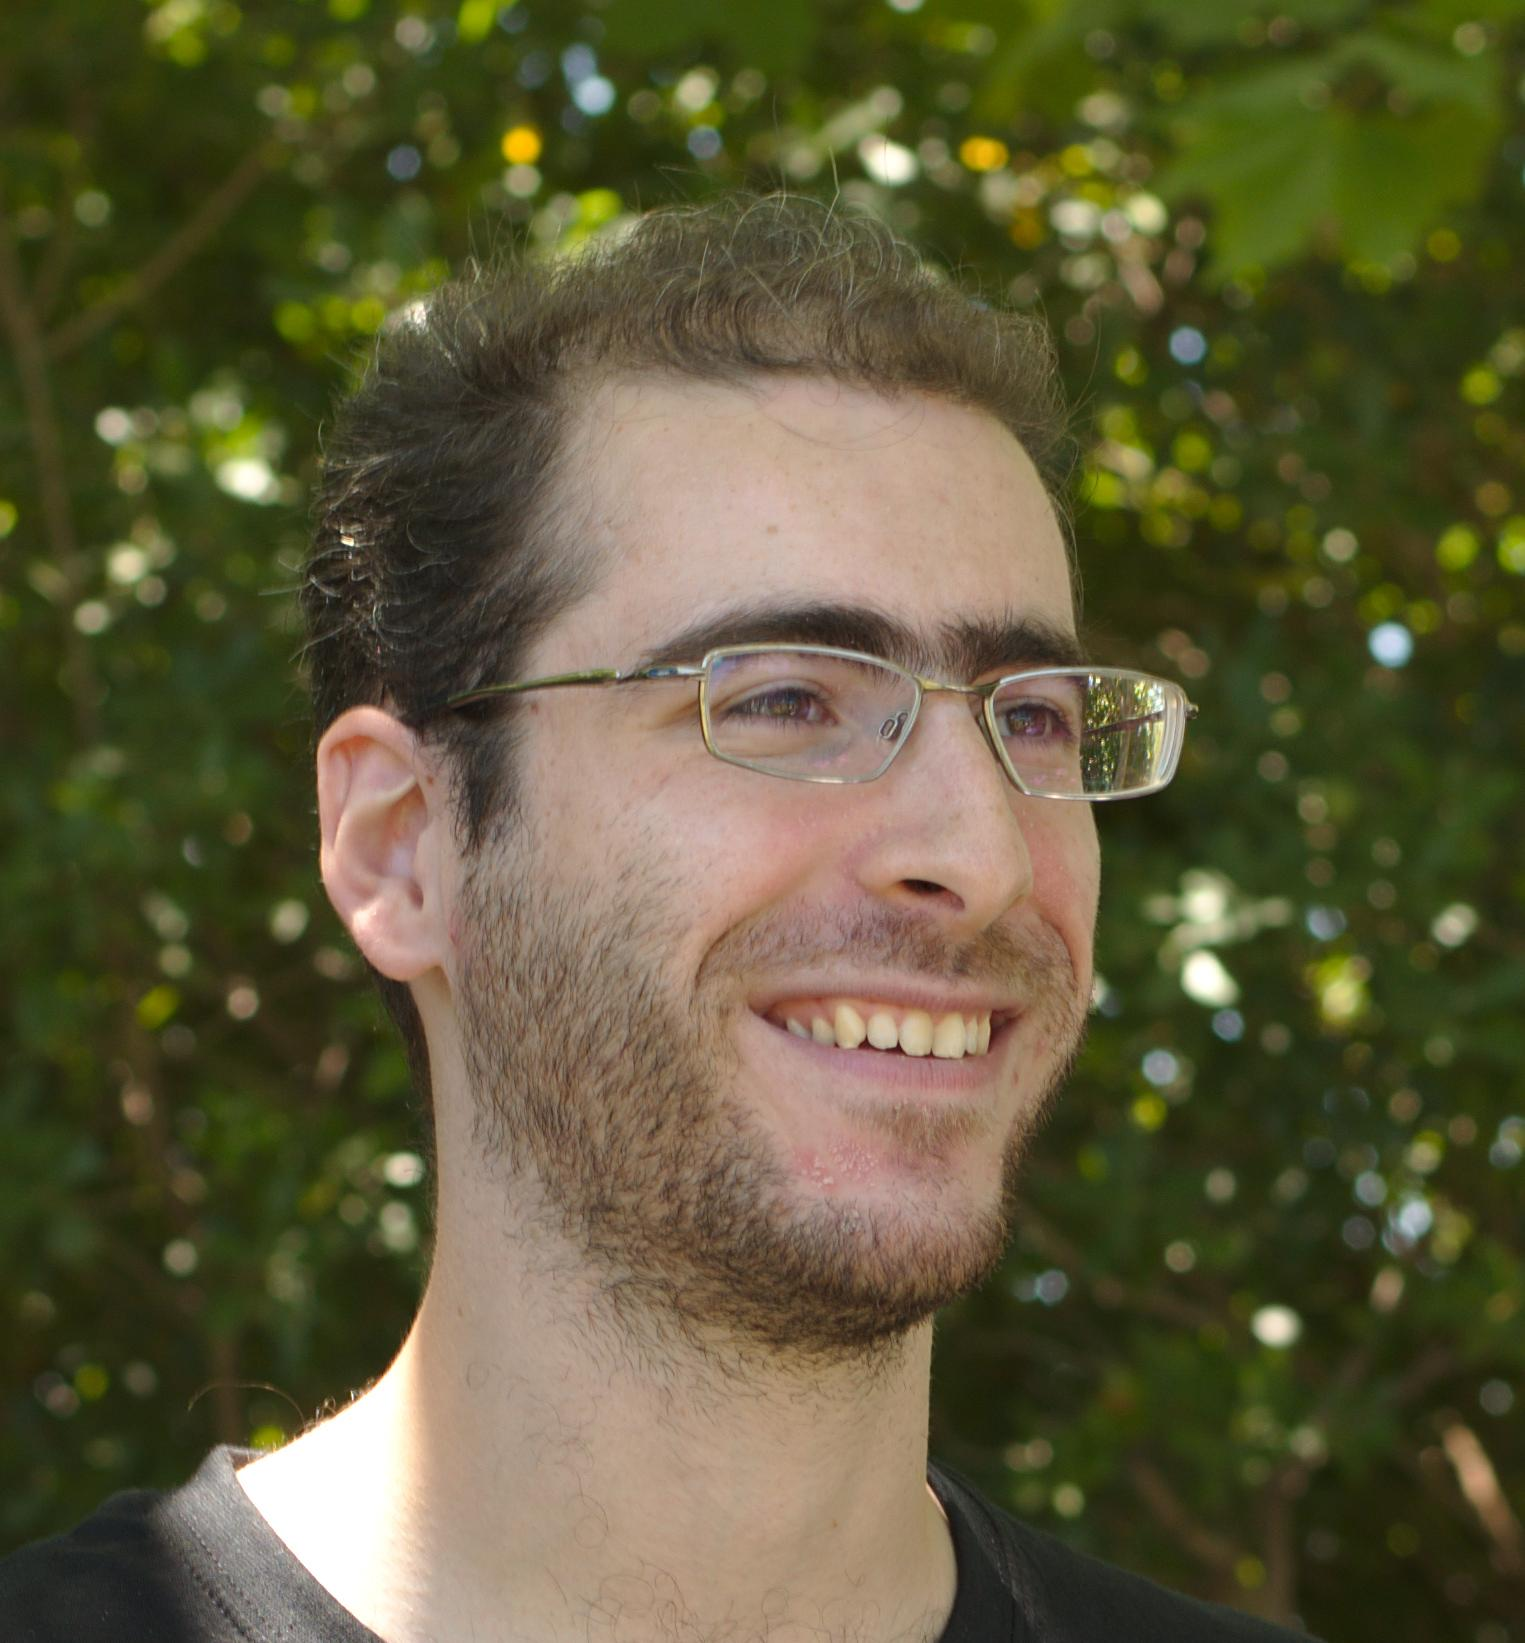
\includegraphics[clip,width=0.2\linewidth]{myfoto.jpg}	%trimming relative to image size!
\end{flushright}
\end{figure}

%---------------------------------------------------------------------------------------
%	QR CODE (optional)
%----------------------------------------------------------------------------------------
%\vspace{-136pt}
%\hspace{0.75\linewidth}
%\includegraphics[width=103pt]{qrcode}
%\normalsize
%\vspace{88pt}

%---------------------------------------------------------------------------------------
%	META SECTION
%----------------------------------------------------------------------------------------

\vspace{-114pt}

\metasection{Fields:}{Distributed Systems, Devops, Software Architecture} 
\metasection{Programming:}{C++, C\#, Python, Rust}
\metasection{Technologies:}{Windows, Linux, Jenkins, AzDevops, Docker, Terraform}
\metasection{Languages:}{English (C1), Portuguese (C2)}

%---------------------------------------------------------------------------------------
%	SUMMARAY (optional)
%----------------------------------------------------------------------------------------

%\cvsection{Summary}\\
%I am a digital media graduate (M.Sc.) with project experience in educational research as well as in the private sector. During my studies I focused on e-assessment software and moved over to b2b software for IBM Notes Domino.

%Currently I develop and evaluate the next generation learning management system with Meteor based on an extensive nursing curriculum for healthcare education.  I also love fitness, martial arts, videogames, news and Sci-Fi series.\\[-2pt]

%============================================================================%
%
%	CV SECTIONS AND EVENTS (MAIN CONTENT)
%
%============================================================================%

\textcolor{softcol}{\hrule}
\vspace{12pt}
As an experienced software engineer, I'm passionate about creating scalable and performant solutions that meet business and technical requirements.

I take pride in writing clean, maintainable, and efficient code, and I am always improving my skills and knowledge. I believe in the importance of code quality and testing, and strive to deliver software that meets or exceeds expectations.

I am committed to identifying technical constraints and opportunities, and design solutions that align with business goals. I am a team player who values my colleagues' ideas and insights, and I am confident that my experience and skills make me a valuable addition to my team.
\vspace{12pt}

%---------------------------------------------------------------------------------------
%	EXPERIENCE
%----------------------------------------------------------------------------------------
\cvsection{Experience}

%
\cvevent{2021 -}{Senior Software Engineer}{OMP}{
	{Designed, developed and maintained a scalable, fault tolerant, self healing caching service used to speedup C++ compilation},
	{Researched how to refactor OMP's supply chain planning solution to scale up and handle the use cases of the largest manufacturing companies in the world}
}

%\textcolor{softcol}{\hrule}

%
\cvevent{2018 - 2021}{Software Engineer}{OMP}{
	{Designed and implemented a high performance event logging framework and introduced observability features to our products},
	{Created CI pipelines}
}

%\textcolor{softcol}{\hrule}

%
\cvevent{2017 - 2018}{Junior Software Engineer}{OMP}{
	{Designed and developed a peer-to-peer file cache to speed up C++ compilation, massively improving build times and boosting developers' productivity},
	{Maintained our in-house development tools and provided support to internal users}
}

%\textcolor{softcol}{\hrule}

%Portugal
\cvevent{2015 - 2017}{Software Engineer}{Altitude Software}{
	{Worked in the R\&D team that develops the back-end of Altitude's distributed call center management software suite capable of handling thousands of calls per minute}
}

%\textcolor{softcol}{\hrule}

%
\cvevent{2014 - 2015}{Apprentice Systems Administrator}{INESC-ID}{
	{Set up automatic installation and configuration of an on-premises machine cluster. Solved technical issues and provided user support}
}

\pagebreak

%---------------------------------------------------------------------------------------
%	EDUCATION SECTION
%--------------------------------------------------------------------------------------

\cvsection{Education}

%\textcolor{softcol}{\hrule}
\cvevent{2012 - 2015}{Master's degree in Distributed Systems and Software Engineering}{Instituto Superior Técnico}{
		{Master Thesis: "Compilation of OpenCL Programs for Stream Processing Architectures": Implemented the OpenCL framework API, a device driver for an FPGA, static code analysis using the LLVM infrastructure, analysis of memory access dependencies in OpenCL kernels, and task scheduling achieving greater speedup}
}

%\textcolor{softcol}{\hrule}

%
\cvevent{2009 - 2012}{Bachelor's degree in Computer Science and Engineering}{Instituto Superior Técnico}{}

%\textcolor{softcol}{\hrule}

%---------------------------------------------------------------------------------------
%	SOFT SKILLS SECTION
%--------------------------------------------------------------------------------------

\cvsection{Soft skills}

\cvevent{}{Coaching}{}{
	{Onboarded and coached new colleagues, guiding them towards becoming higher quality programmers and overall better engineers}
}

\cvevent{}{Leadership}{}{
	{Training about positioning as a leader, manager and coach, situational leadership, dealing with change, commitment, trust, accountability and results}
	%{Positioning as a leader, manager and coach},
	%{Situational leadership},
	%{Dealing with change, commitment, trust, accountability and results}
}

\cvevent{}{Communication}{}{
	{Training about communication style and the effect on others, active listening and open dialogue, giving and receiving feedback, improving teamwork through effective meetings, customer centric behavior, empathy and communication with customers}
	%{Communication style and the effect on others},
	%{Active listening and open dialogue},
	%{Giving and receiving feedback},
	%{Improving teamwork through effective meetings},
	%{Customer centric behavior, empathy and communication with customers}
}

%--------------------------------------------------------------------------------------
\cvsection{Informal education}

\cvevent{}{iLean Agile Workshop}{}{
	{Agile mindset and implementing Agile and Lean techniques. Stakeholders, roles, scrum events, estimations, sprints and backlog}
}

\cvevent{}{Recently read}{}{
	{Kubernetes: Up and Running, 3rd Edition, \textit{by Brendan Burns, Joe Beda, Kelsey Hightower, Lachlan Evenson}},
	{Designing Data-Intensive Applications, \textit{by Martin Kleppmann}},
	{Software Architecture: The Hard Parts, \textit{by Neal Ford, Mark Richards, Pramod Sadalage, Zhamak Dehghani}},
	{Designing Distributed Systems, \textit{by Brendan Burns}}
}

%-------------------------------------------------------------------------------------------------
%	ARTIFICIAL FOOTER (fancy footer cannot exceed linewidth) 
%--------------------------------------------------------------------------------------------------

\null
\vspace*{\fill}
\hspace{-0.25\linewidth}\colorbox{bgcol}{\makebox[1.5\linewidth][c]{\mystrut \small \textcolor{white}{} $\cdot$ \textcolor{white}{}}}




%============================================================================%
%
%
%
%	DOCUMENT END
%
%
%
%============================================================================%
\end{document}
